\documentclass[12pt,a4paper]{article}

% ============================================================================
% PACKAGES
% ============================================================================
\usepackage[utf8]{inputenc}
\usepackage[T1]{fontenc}
\usepackage[margin=1in,headheight=14.5pt]{geometry}
\usepackage{graphicx}
\usepackage{float}
\usepackage{amsmath,amssymb,amsthm}
\usepackage{booktabs}
\usepackage{caption}
\usepackage{subcaption}
\usepackage{hyperref}
\usepackage{cleveref}
\usepackage{listings}
\usepackage{xcolor}
\usepackage{fancyhdr}
\usepackage{titlesec}
\usepackage{abstract}
\usepackage{enumitem}
\usepackage{tikz}
\usepackage{pgfplots}
\pgfplotsset{compat=1.18}
\usepackage{natbib}
\usepackage{appendix}
\usepackage{tocloft}

% ============================================================================
% HYPERREF SETUP
% ============================================================================
\hypersetup{
    colorlinks=true,
    linkcolor=blue,
    filecolor=magenta,
    urlcolor=cyan,
    citecolor=blue,
    pdftitle={Report Title},
    pdfauthor={Author Name},
    bookmarks=true,
}

% ============================================================================
% CODE LISTING SETUP
% ============================================================================
\lstset{
    basicstyle=\ttfamily\small,
    keywordstyle=\color{blue}\bfseries,
    commentstyle=\color{green!60!black},
    stringstyle=\color{orange},
    showstringspaces=false,
    numbers=left,
    numberstyle=\tiny\color{gray},
    stepnumber=1,
    numbersep=8pt,
    frame=single,
    breaklines=true,
    breakatwhitespace=true,
    tabsize=4,
    captionpos=b
}

% ============================================================================
% HEADER AND FOOTER
% ============================================================================
\pagestyle{fancy}
\fancyhf{}
\fancyhead[L]{\leftmark}
\fancyhead[R]{\thepage}
\fancyfoot[C]{\small \textit{Report Title}}
\renewcommand{\headrulewidth}{0.4pt}
\renewcommand{\footrulewidth}{0.4pt}

% ============================================================================
% SECTION FORMATTING
% ============================================================================
\titleformat{\section}
  {\normalfont\Large\bfseries}{\thesection}{1em}{}
\titleformat{\subsection}
  {\normalfont\large\bfseries}{\thesubsection}{1em}{}
\titleformat{\subsubsection}
  {\normalfont\normalsize\bfseries}{\thesubsubsection}{1em}{}

% ============================================================================
% THEOREM ENVIRONMENTS
% ============================================================================
\theoremstyle{definition}
\newtheorem{definition}{Definition}[section]
\newtheorem{theorem}{Theorem}[section]
\newtheorem{lemma}{Lemma}[section]
\newtheorem{corollary}{Corollary}[section]
\newtheorem{proposition}{Proposition}[section]
\newtheorem{example}{Example}[section]
\newtheorem{remark}{Remark}[section]

% ============================================================================
% CUSTOM COMMANDS
% ============================================================================
\newcommand{\R}{\mathbb{R}}
\newcommand{\N}{\mathbb{N}}
\newcommand{\Z}{\mathbb{Z}}
\newcommand{\Q}{\mathbb{Q}}
\newcommand{\E}{\mathbb{E}}
\newcommand{\Var}{\text{Var}}
\newcommand{\Cov}{\text{Cov}}
\newcommand{\Corr}{\text{Corr}}

% ============================================================================
% TITLE PAGE INFORMATION
% ============================================================================
\title{
    \vspace{2cm}
    \textbf{\LARGE Report Title}\\
    \vspace{0.5cm}
    \large Subtitle or Course Code\\
    \vspace{1.5cm}
}
\author{
    \textbf{Author Name}\\
    Student ID: 123456789\\
    \vspace{0.5cm}
    Department of Mathematics \& Statistics\\
    University Name\\
    \vspace{0.5cm}
    \texttt{email@university.edu}
}
\date{\today}

% ============================================================================
% DOCUMENT BEGINS
% ============================================================================
\begin{document}

% ============================================================================
% TITLE PAGE
% ============================================================================
\begin{titlepage}
    \centering
    \vspace*{1cm}

    % \includegraphics[width=0.3\textwidth]{university_logo.png}\\[1cm]
    % Remove or comment out the line above if you don't have a logo

    \vspace{1cm}

    {\Huge\bfseries Report Title\par}
    \vspace{0.5cm}
    {\Large Subtitle or Course Code\par}

    \vspace{2cm}

    {\Large\textbf{Author Name}\par}
    \vspace{0.3cm}
    {\large Student ID: 123456789\par}

    \vspace{1.5cm}

    {\large Department of Mathematics \& Statistics\\
    University Name\par}

    \vspace{1cm}

    {\large \texttt{email@university.edu}\par}

    \vfill

    {\large Submitted to: Professor Name\par}
    \vspace{0.3cm}
    {\large Course: COURSE CODE - Course Name\par}

    \vfill

    {\large \today\par}

\end{titlepage}

% ============================================================================
% ABSTRACT
% ============================================================================
\newpage
\begin{abstract}
\noindent
This is the abstract section where you provide a brief summary of the report.
It should concisely describe the problem, methodology, key findings, and conclusions.
Typically, an abstract is 150-300 words and provides readers with a quick overview
of the entire document without needing to read the full text. Include the main
objectives, approach, results, and implications of your work.
\end{abstract}

\vspace{1cm}

\noindent\textbf{Keywords:} Keyword1, Keyword2, Keyword3, Keyword4, Keyword5

% ============================================================================
% TABLE OF CONTENTS
% ============================================================================
\newpage
\tableofcontents
\newpage

% Optional: List of Figures and Tables
\listoffigures
\newpage
\listoftables
\newpage

% ============================================================================
% MAIN CONTENT
% ============================================================================

\section{Introduction}
\label{sec:introduction}

This is the introduction section where you present the background, motivation,
and objectives of your report. Introduce the problem you are addressing, provide
relevant context, and outline the structure of the document.

\subsection{Background and Motivation}
\label{subsec:background}

Provide background information about the topic. Why is this research important?
What gap in knowledge does it address?

\subsection{Research Objectives}
\label{subsec:objectives}

Clearly state the main objectives of your research or assignment:
\begin{enumerate}
    \item First objective
    \item Second objective
    \item Third objective
\end{enumerate}

\subsection{Report Structure}
\label{subsec:structure}

Briefly describe the organization of the report. For example:
\Cref{sec:literature} reviews relevant literature,
\Cref{sec:methodology} describes the methodology,
\Cref{sec:results} presents the results, and
\Cref{sec:conclusion} concludes the report.

% ============================================================================
\section{Literature Review}
\label{sec:literature}

Review existing research and literature relevant to your topic. Cite sources
using \texttt{natbib} package commands like \citet{author2020} or \citep{author2020}.

\subsection{Theoretical Framework}
\label{subsec:theory}

Discuss the theoretical foundations of your work.

\begin{definition}[Bond Price]
\label{def:bond_price}
The price of a bond is the present value of its future cash flows, discounted
at the appropriate yield to maturity.
\end{definition}

\subsection{Related Work}
\label{subsec:related_work}

Summarize key findings from related studies and how they relate to your work.

% ============================================================================
\section{Methodology}
\label{sec:methodology}

Describe the methods, models, and techniques you used in your research or assignment.

\subsection{Data Description}
\label{subsec:data}

Describe the data sources, collection methods, and preprocessing steps.

\begin{table}[H]
\centering
\caption{Summary Statistics of Dataset}
\label{tab:summary_stats}
\begin{tabular}{@{}lcccc@{}}
\toprule
Variable & Mean & Std. Dev. & Min & Max \\
\midrule
Variable 1 & 10.5 & 2.3 & 5.0 & 15.0 \\
Variable 2 & 8.7 & 1.8 & 4.0 & 12.0 \\
Variable 3 & 15.2 & 3.1 & 8.0 & 22.0 \\
\bottomrule
\end{tabular}
\end{table}

\subsection{Mathematical Model}
\label{subsec:model}

Present the mathematical formulation of your model.

\begin{equation}
\label{eq:bond_price}
P = \sum_{t=1}^{n} \frac{C}{(1+y)^t} + \frac{F}{(1+y)^n}
\end{equation}

where $P$ is the bond price, $C$ is the coupon payment, $y$ is the yield to maturity,
$F$ is the face value, and $n$ is the number of periods.

\begin{theorem}[Present Value Theorem]
\label{thm:pv}
The present value of a series of cash flows $\{CF_t\}_{t=1}^{n}$ discounted at rate $r$ is:
\begin{equation}
PV = \sum_{t=1}^{n} \frac{CF_t}{(1+r)^t}
\end{equation}
\end{theorem}

\begin{proof}
The proof follows from the time value of money principle...
\end{proof}

\subsection{Implementation}
\label{subsec:implementation}

Describe how you implemented your methodology. Include code snippets if relevant.

\begin{lstlisting}[language=Python, caption=Bond Pricing Implementation, label=lst:bond_price]
import numpy as np

def price_bond(coupon, yield_rate, maturity, face_value=100):
    """Calculate bond price given coupon, yield, and maturity."""
    periods = np.arange(1, maturity + 1)
    coupon_pv = np.sum(coupon / (1 + yield_rate) ** periods)
    principal_pv = face_value / (1 + yield_rate) ** maturity
    return coupon_pv + principal_pv
\end{lstlisting}

% ============================================================================
\section{Results and Analysis}
\label{sec:results}

Present your findings with tables, figures, and analysis.

\subsection{Empirical Results}
\label{subsec:empirical}

\begin{figure}[H]
    \centering
    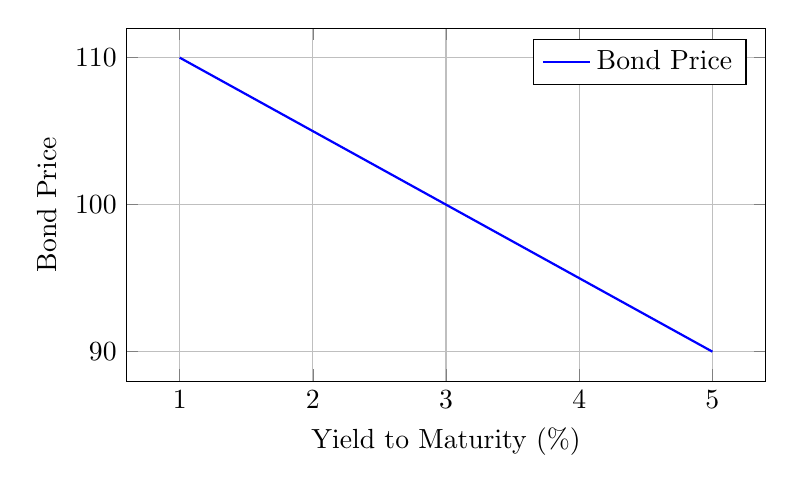
\begin{tikzpicture}
        \begin{axis}[
            xlabel={Yield to Maturity (\%)},
            ylabel={Bond Price},
            width=0.8\textwidth,
            height=0.5\textwidth,
            grid=major,
            legend pos=north east
        ]
        \addplot[blue, thick] coordinates {
            (1, 110) (2, 105) (3, 100) (4, 95) (5, 90)
        };
        \legend{Bond Price}
        \end{axis}
    \end{tikzpicture}
    \caption{Relationship between Yield and Bond Price}
    \label{fig:yield_price}
\end{figure}

As shown in \Cref{fig:yield_price}, there is an inverse relationship between
yield to maturity and bond price, consistent with the theoretical model in
\Cref{eq:bond_price}.

\subsection{Statistical Analysis}
\label{subsec:stats}

Conduct statistical tests and report the results.

\begin{table}[H]
\centering
\caption{Regression Results}
\label{tab:regression}
\begin{tabular}{@{}lcccc@{}}
\toprule
Variable & Coefficient & Std. Error & t-statistic & p-value \\
\midrule
Intercept & 5.234 & 0.123 & 42.52 & <0.001 \\
Yield & -2.145 & 0.045 & -47.67 & <0.001 \\
Maturity & 0.321 & 0.012 & 26.75 & <0.001 \\
\midrule
$R^2$ & \multicolumn{4}{c}{0.892} \\
\bottomrule
\end{tabular}
\end{table}

\subsection{Discussion}
\label{subsec:discussion}

Interpret the results and discuss their implications. Compare with existing
literature and theoretical predictions.

% ============================================================================
\section{Conclusion}
\label{sec:conclusion}

Summarize the main findings of your report and their implications.

\subsection{Summary of Findings}
\label{subsec:summary}

\begin{itemize}
    \item Finding 1: Brief description
    \item Finding 2: Brief description
    \item Finding 3: Brief description
\end{itemize}

\subsection{Limitations}
\label{subsec:limitations}

Acknowledge any limitations of your study:
\begin{enumerate}
    \item Data limitations
    \item Methodological constraints
    \item Scope restrictions
\end{enumerate}

\subsection{Future Research}
\label{subsec:future}

Suggest directions for future research based on your findings.

% ============================================================================
% ACKNOWLEDGMENTS (Optional)
% ============================================================================
\section*{Acknowledgments}
\addcontentsline{toc}{section}{Acknowledgments}

I would like to thank Professor Name for their guidance and support throughout
this project. I also acknowledge the helpful discussions with colleagues and
the financial support from Institution Name.

% ============================================================================
% BIBLIOGRAPHY
% ============================================================================
\newpage
\bibliographystyle{apalike}
\bibliography{references}
% Create a references.bib file with your bibliography entries
% Example entry:
% @article{author2020,
%   author = {Author, A.},
%   title = {Title of Paper},
%   journal = {Journal Name},
%   year = {2020},
%   volume = {10},
%   pages = {123--145}
% }

% ============================================================================
% APPENDICES
% ============================================================================
\newpage
\begin{appendices}

\section{Additional Derivations}
\label{app:derivations}

Include additional mathematical derivations or proofs that are too detailed
for the main text.

\section{Data Tables}
\label{app:data}

Include additional data tables or detailed results.

\begin{table}[H]
\centering
\caption{Complete Dataset}
\label{tab:complete_data}
\begin{tabular}{@{}lcccc@{}}
\toprule
ID & Variable 1 & Variable 2 & Variable 3 & Variable 4 \\
\midrule
1 & 10.5 & 8.7 & 15.2 & 20.1 \\
2 & 11.2 & 9.1 & 16.0 & 21.5 \\
3 & 9.8 & 8.2 & 14.5 & 19.3 \\
\bottomrule
\end{tabular}
\end{table}

\section{Code Listings}
\label{app:code}

Include complete code implementations.

\begin{lstlisting}[language=Python, caption=Complete Analysis Script]
import numpy as np
import pandas as pd
import matplotlib.pyplot as plt

# Your complete code here
\end{lstlisting}

\end{appendices}

\end{document}
